\newpage
\section{Dataset building}
\label{section:datasetChapter}
Since the objective of this thesis is to generate a realistic photo of a face starting from a handmade sketch, a neural network had to be trained on a large dataset of face images and their corresponding sketches. However, finding such a dataset is not easy. Online there is available the \href{http://mmlab.ie.cuhk.edu.hk/archive/facesketch.html}{CUHK dataset} (The Chinese University of Hong Kong), it is a collection of images and annotations used for various computer vision and machine learning tasks, such as image classification, object detection, and face recognition. The specific content and size of the CUHK dataset may vary depending on the source. It is often used as a benchmark for evaluating and comparing the performance of different algorithms in various computer vision tasks. The dataset includes the CUHK Face Sketch FERET Database (CUFSF) which is composed of a pair of images with both a photo of a face and a sketch of it. Each face in the database includes an artist-drawn sketch based on a photo that was taken with the individual in a neutral expression, under normal lighting conditions, and in a frontal pose. This database is made for the purpose of researching face sketch synthesis and face sketch recognition. Unluckily, it does not contain enough images, and it requires data augmentation techniques in order to use it.  \\
Another dataset available online is the \href{https://github.com/NVlabs/ffhq-dataset}{FFHQ} (Flickr-Faces-HQ) dataset, which is a large-scale, high-quality dataset of face images, created to advance research in generative models and computer vision. The dataset contains $70,000$ high-resolution (1024×1024) images of diverse human faces, each with different poses, lighting, expressions, and ethnicities. Since it is a very large dataset, it can be used to create the needed dataset composed of the pairs of sketches and photos, but it requires some image processing techniques in order to obtain the sketches.

\noindent The challenge here is to find a technique to transform an image into a sketch. The idea is to extract the face contours using an edge detection technique while preserving the essential details of the face and making the extracted  a hand-drawn sketch appearance

\noindent To achieve these results, two approaches were considered to build the dataset. The first approach involves using the \href{https://github.com/vijishmadhavan/ArtLine}{Artline} network and the Learning to Simplify network \cite{SketchSimplify}. The second approach involves using an extended difference of Gaussian (XDoG) edge detector \cite{xdog} and the Learning to Simplify network.
In order to produce the desired results, both approaches need to be carefully analysed and compared. In this way, the most appropriate approach can be chosen and further developed to create a realistic handmade sketch. 
Now will follow an introduction of the above approaches before discussing how they have been used to reach the final goal.

\subsection{Artline}
Artline is a deep neural network designed specifically to turn photographs into line art drawings. It is a recent project developed by a developer interested in generative modelling, that follows the discoveries found by Jason Antic, another developer, in his \href{https://github.com/jantic/DeOldify}{DeOldify} project, utilising advancements and tools developed by the team at Fast.ai. Artline, as DeOldify, is based on a self-attention GAN (SAGAN) that is progressively resized to achieve a desired resolution. SAGAN was introduced in a 2018 research paper by Zhang et al.\cite{SaGAN} and has since been applied to a wide range of image generation tasks, including facial image synthesis, artistic image generation, and more. The results have been very promising, with SAGAN producing high-quality and highly detailed images that are comparable to those produced by state-of-the-art methods. \\
The self-attention mechanism allows the generator network to weigh the contribution of different parts of an image in generating the final result. This allows the network to focus on important features of the image and produce more accurate results. Additionally, the use of self-attention also allows the network to better capture the relationships between different parts of the image, resulting in more coherent and visually appealing images.
Artline has been trained on the APDrawing dataset, which is a dataset obtained from another generative neural network able to generate high-quality sketch drawings from a given image, called APDrawingGAN \cite{APDrawingGAN}. The APDrawingGAN is an innovative GAN-based architecture that has the capability to generate professional-level artistic portraits. It uses a combination of a global network and local networks, which allows for dedicated drawing strategies to be learned for specific facial features. This leads to a more precise and accurate portrayal of facial features in the generated drawings. To train APDrawingGAN, a unique artistic drawing dataset was constructed, containing high-resolution portrait photos and corresponding professional artistic drawings. The results of extensive experiments and a user study demonstrate that APDrawingGAN produces significantly better artistic drawings than existing methods. Since the results obtained by the authors using this dataset were good only in the case of ID photos, the authors combined this dataset with an Anime sketch dataset to obtain good results also with other kinds of pictures.

\subsection{Learning to simplify}
Learning to Simplify is a model which consists of a fully convolutional network (FCN) to learn the mapping between rough sketches and clean drawings. The technique of simplifying rough sketches utilises Convolutional Neural Networks (CNNs) to simplify the image. Through a series of convolution operations, the sketch lines are grouped, and a simplification is directly produced. The CNNs are trained using a unique dataset of rough sketches and their corresponding simplifications, which the authors have created. This data-driven method has several benefits. Firstly, the model automatically learns the necessary heuristics for sketch simplification from the training data. Secondly, convolution operations can be executed efficiently on GPUs, resulting in processing times of less than a second for most images. In contrast to typical CNN architectures, which utilise fully connected layers, their approach uses solely convolutional layers. These sparse connections allow their CNN to process images of varying resolutions and aspect ratios with ease. The results of the study show that the FCN is able to produce high-quality clean drawings from rough sketches with remarkable accuracy.
\begin{figure}[h!]
\centering
  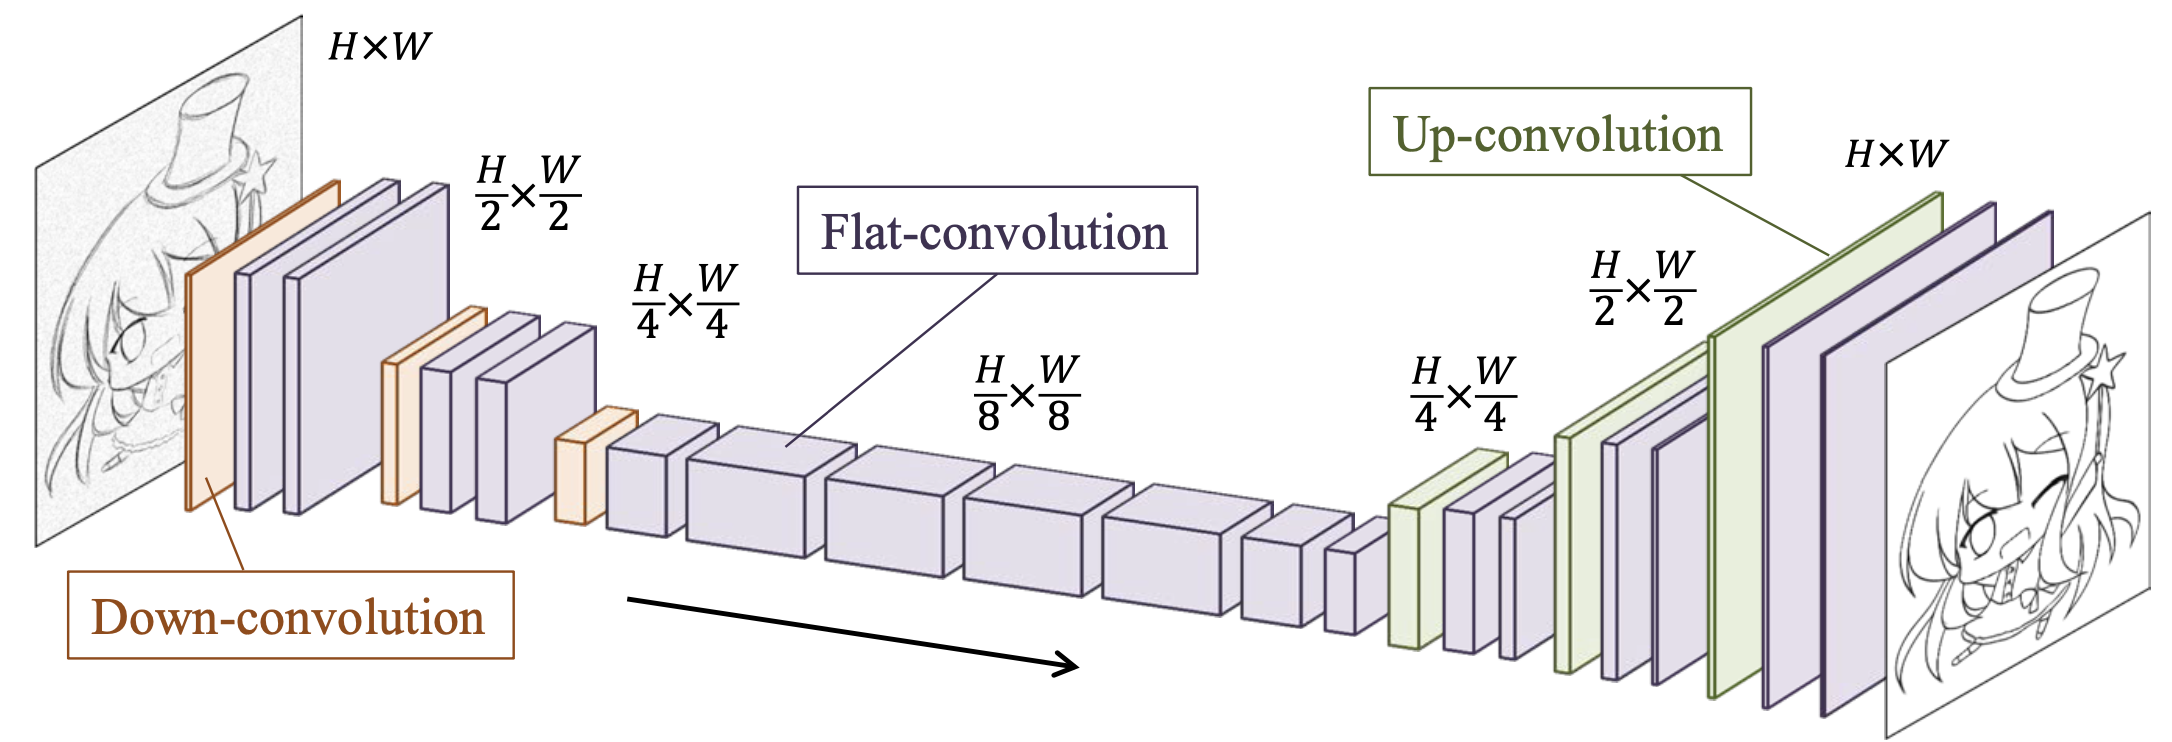
\includegraphics[scale=0.35]{figures/learnToSimplifyArchitecture.png}
  \caption{Learning to Simplify architecture. Image taken from \cite{SketchSimplify}}
  \label{fig:Learning to Simplify architecture}
\end{figure}
\\
The model has three main components: an encoder that compresses the image, a processing unit that extracts the critical lines, and a decoder that converts the simplified representation back into a greyscale image of the same resolution as the input (Figure \ref{fig:Learning to Simplify architecture}). All these components use convolutional layers for their processing.


\noindent The model uses a down- and up-convolution architecture that may look like simple filter banks. However, the model has a larger number of channels in lower-resolution parts, such as 1024 channels when the size is 1/8, to ensure that the necessary information for clean lines is carried through. The model uses padding in its convolutional layers to ensure the output is the same size as the input when a stride of 1 is used. Instead of pooling layers, they used convolutional layers with a higher stride to lower the resolution from the previous layer. To increase the resolution and ensure that the output of the model has the same dimensions as the input, they used fractional strides.
Overall, the model leverages the ability of CNNs to learn and extract essential information, making it an effective solution for sketch simplification.
The Learn to simplify model has been trained by the authors using pairs of rough and simplified sketches representing the input and the target, respectively.
An example of the results that can be obtained with this approach can be seen in fig. \ref{fig:Learning to Simplify results}.
\begin{figure}[htbp]
\centering
  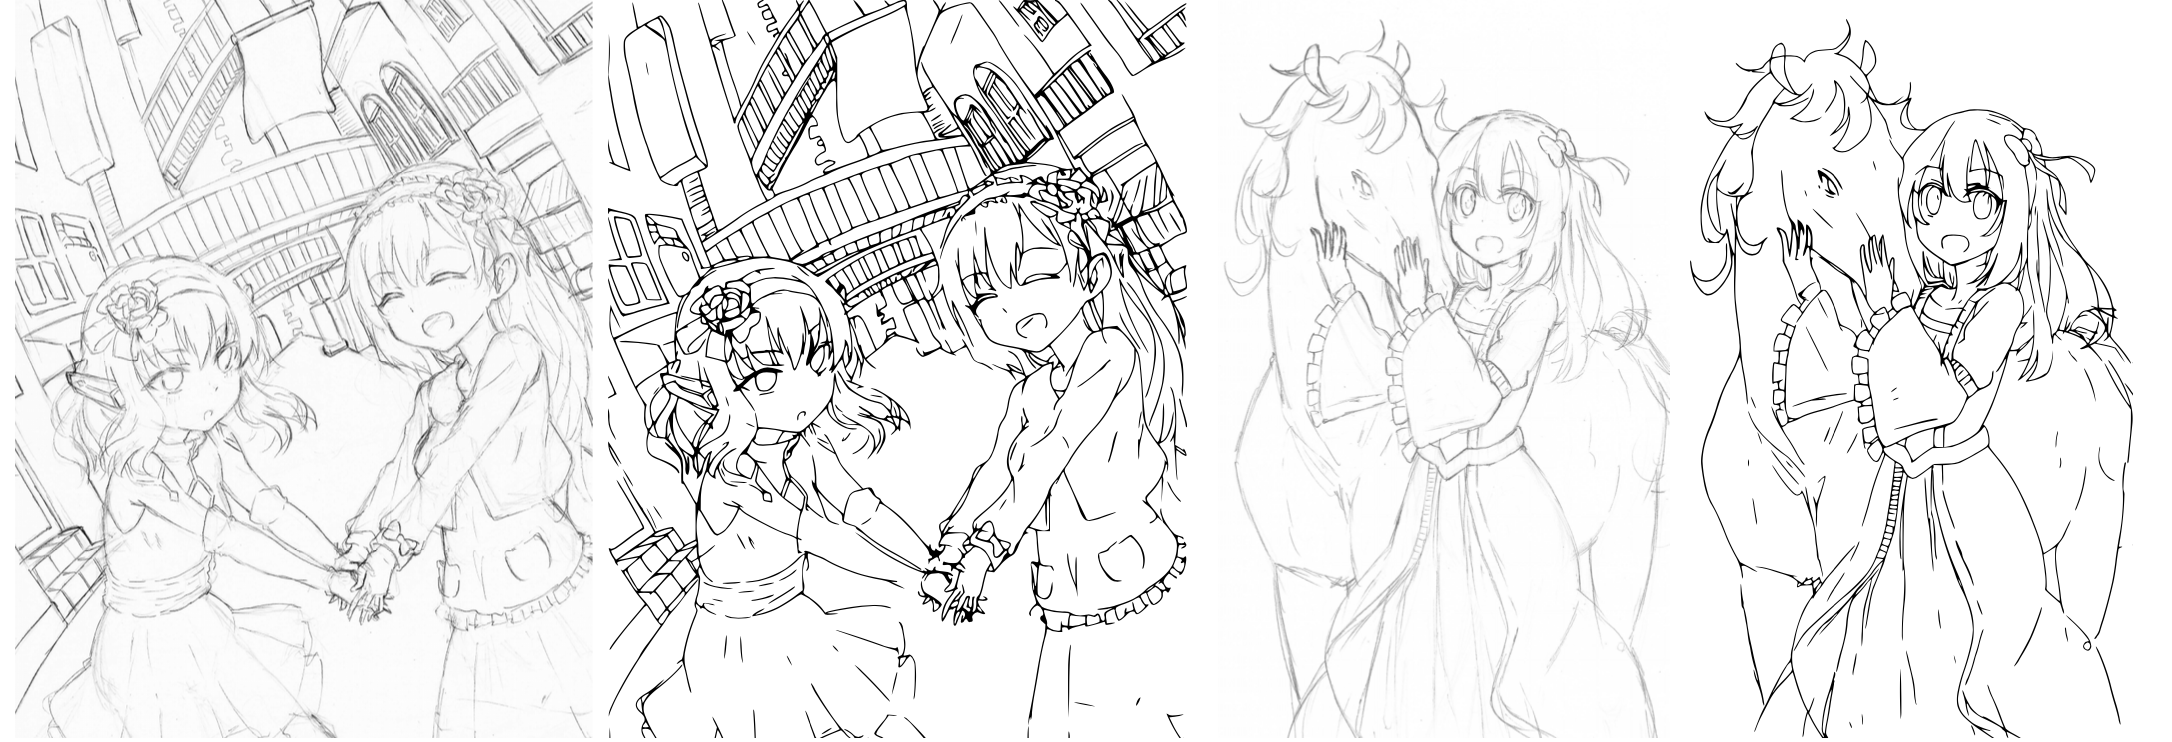
\includegraphics[scale=0.25]{figures/learnToSimplify-results-paper.png}
  \caption{Figure from \cite{SketchSimplify}} showing the results of Learning to Simplify approach.
  \label{fig:Learning to Simplify results}
\end{figure}

\subsection{Extended Difference of Gaussian (XDoG)}
The Extended Difference of Gaussian (XDoG) is an edge detector operator based on the Difference of Gaussian (DoG). The Difference of Gaussian is based on the idea that edges in an image correspond to rapid changes in intensity, which can be detected by subtracting two images that have been smoothed with different Gaussian kernels. It can be used to increase the visibility of edges and other features in digital images.
The capacity of the DoG operator to extract information about the edges in the image can be explained by considering the Gaussian filter from a signal processing point of view. The Gaussian filter is defined as: 
\begin{equation}
    G_{\sigma}(x)=\frac{1}{2\pi \sigma^2}e^{-\frac{x^2}{2\sigma^2}}
\end{equation}
where $x$ refers to a two-dimensional coordinate, and $\sigma$ represents the standard deviation of the Gaussian distribution in the spatial domain. It is a low-pass filter which attenuates or eliminates high frequencies. The difference between the two Gaussian with different is equivalent to a subtraction between a blurred version of the original image and a less blurred version of it, and it is defined as: 
 \begin{equation}
     D_{\sigma, k}(x)=G_{\sigma}(x)-G_{k\sigma}(x) \approx -(k-1)\sigma^2 \nabla ^2 G
 \end{equation}
where the standard deviations of these Gaussian filters determine the scale at which edges are detected, with larger standard deviations detecting larger edges.
This difference is a band-pass filter which attenuates all frequencies between the cut-off frequencies of the two Gaussians and results in a new image that highlights regions of the original image where the intensity changes rapidly.

\noindent The XDoG approach is inspired by biological models proposed by Young and others \cite{GaussianDerivativeModel}, which were based on the DoG model. Winnem$\ddot o$ller et al. \cite{RealTimeVideoAbstraction} extended the DoG model to allow for greater control over the inhibitory effect of the larger Gaussian, which is allowed to vary, resulting in a more advanced edge detection technique with the following equation:
\begin{equation}
    D_{\sigma, k,\tau}(x)=G_{\sigma}(x)-\tau \cdot G_{k\sigma}(x)
    \label{eq:xdog}
\end{equation}
 This allows for more fine-grained control over the output, resulting in more precise edge detection and image stylization. In particular, it is possible to achieve a wider range of stylistic effects using the following continuous ramp function:
 \begin{equation}
     T_{\epsilon, \varphi}(u) = 
     \begin{cases}
        1 & u \ge \epsilon \\
        1+ \tanh (\varphi \cdot (u-\epsilon)) & \mbox{otherwise}
    \end{cases}
\label{eq:xdog1}
 \end{equation}
Equations \ref{eq:xdog} and \ref{eq:xdog1} taken together is referred to as the XDoG filter $T_{\epsilon, \varphi}(D_{\sigma, k, \tau }*I)$ for a given image $I$. 

\noindent There are a lot of known edge detectors that can be applied to find the edges of objects present in an image, and they have their advantages and disadvantages (as shown in \cite{xdog}). Since the objective was not only to extract contours but also to obtain something that looks like a sketch done by an artist, not all the edge detectors that are known could be applied. 

\noindent As can be seen from figure \ref{fig:xdog-paperComparison}, some edge detectors work well in extracting edges, like the Sobel filter and the Canny edge detector, but the results obtained are not satisfactory from an artistic point of view. Hence, the XDoG operator has been chosen since it satisfies the final purpose.

\begin{figure}[htbp]
\centering
  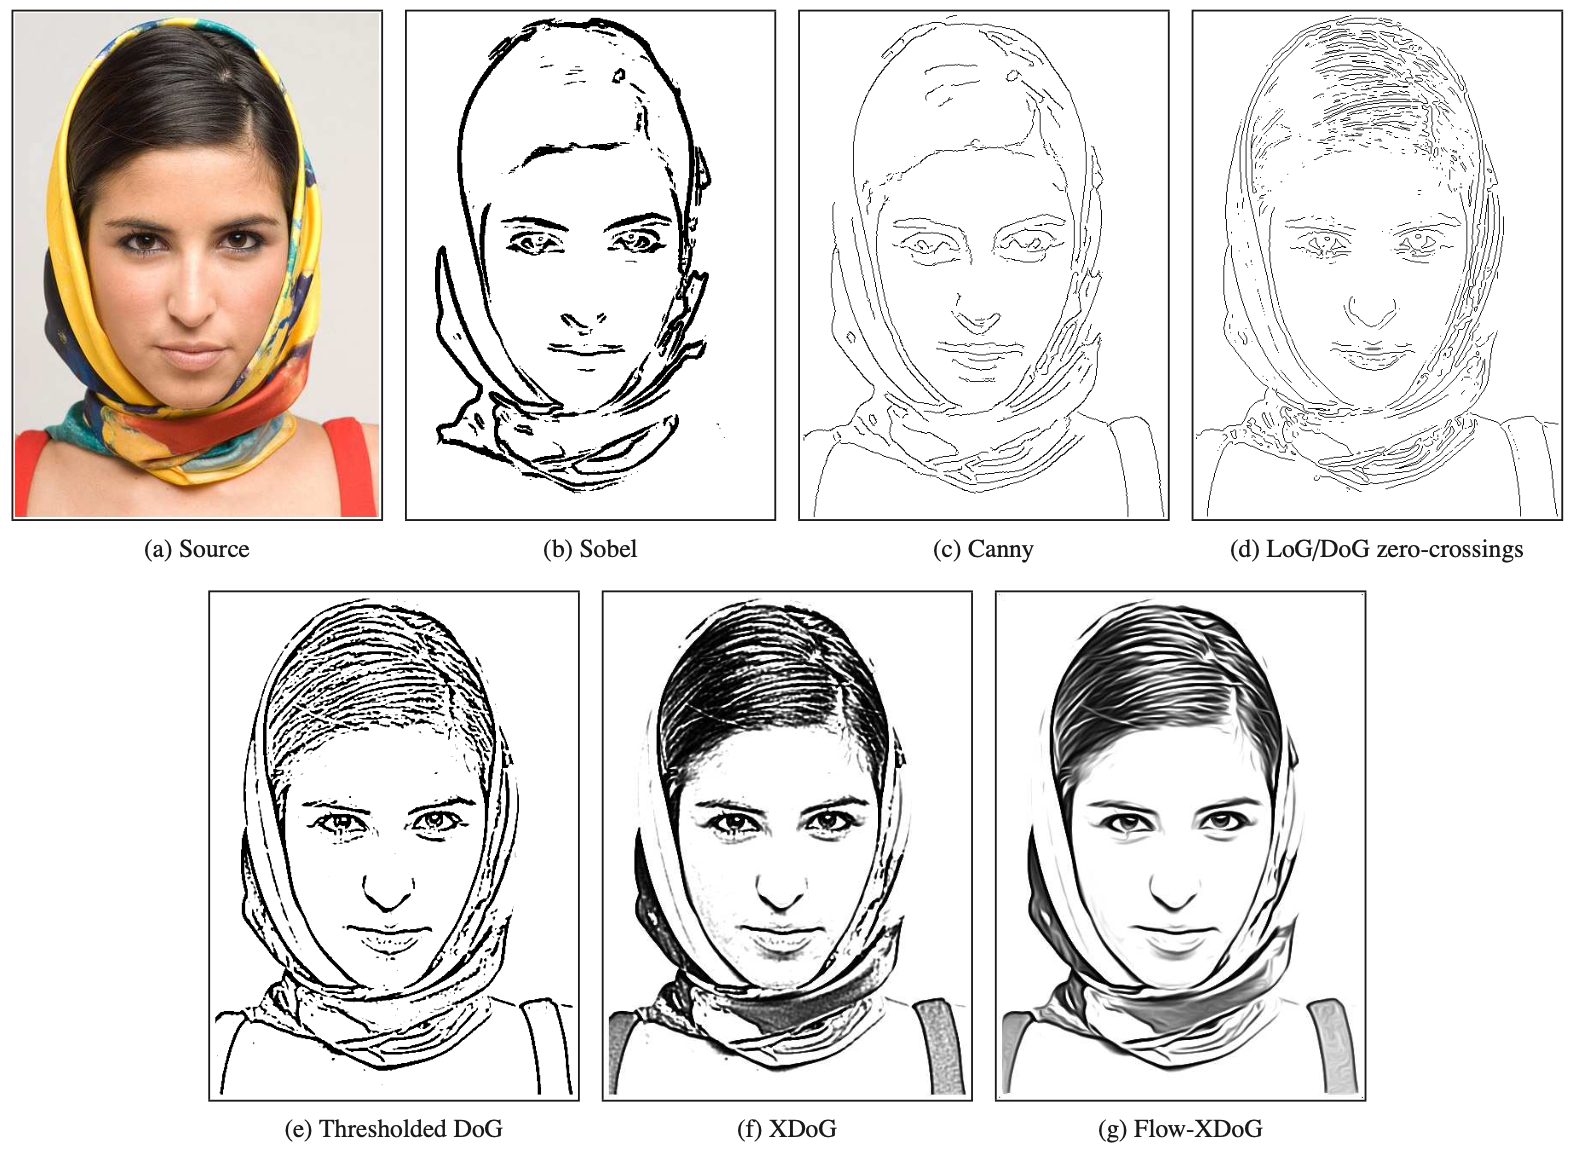
\includegraphics[scale=0.4]{figures/comparisonOfEdgeDetectors.png}
  \caption{Figure taken from \cite{xdog} in which there is a comparison between different known edge detection techniques.}
  \label{fig:xdog-paperComparison}
\end{figure}

\subsection{Implementation (??)}
In order to achieve the needed dataset, the following approaches have been followed:
\begin{enumerate}
    \item Artline network + Learning to Simplify network
    \item extended difference of Gaussian (XDoG) edge detector + Learning to Simplify network
\end{enumerate}
The first idea was to take the images and extract the contours using Artline neural network and then simplify the result by removing some lines from the obtained sketch.
The results obtained applying only Artline can be seen in Fig. \ref{fig:artlineRes}, they are very good and give the impression that they are made by an artist. Nevertheless, they do not seem like sketches made with a pencil because all the people's hair and facial hair are coloured in black. Therefore, there was a need to try to simplify these images, by applying sketch simplification which can be obtained thanks to Learning to Simplify. This network can be used with four different models that are available and can be used to achieve different results.
\noindent The models are:
\begin{itemize}
    \item a model obtained from training the network using only MSE loss
    \item a model obtained from training the network using MSE and GAN loss
    \item a model for pencil drawing generation based on an artist with a dirty and faded pencil style (pencil1)
    \item model for pencil drawing generation based on an artist with a clearer overlay pencil style (pencil2)
\end{itemize}
\begin{figure}[htbp]
    \centering
    \subfloat[][\emph{Original imag}]
    {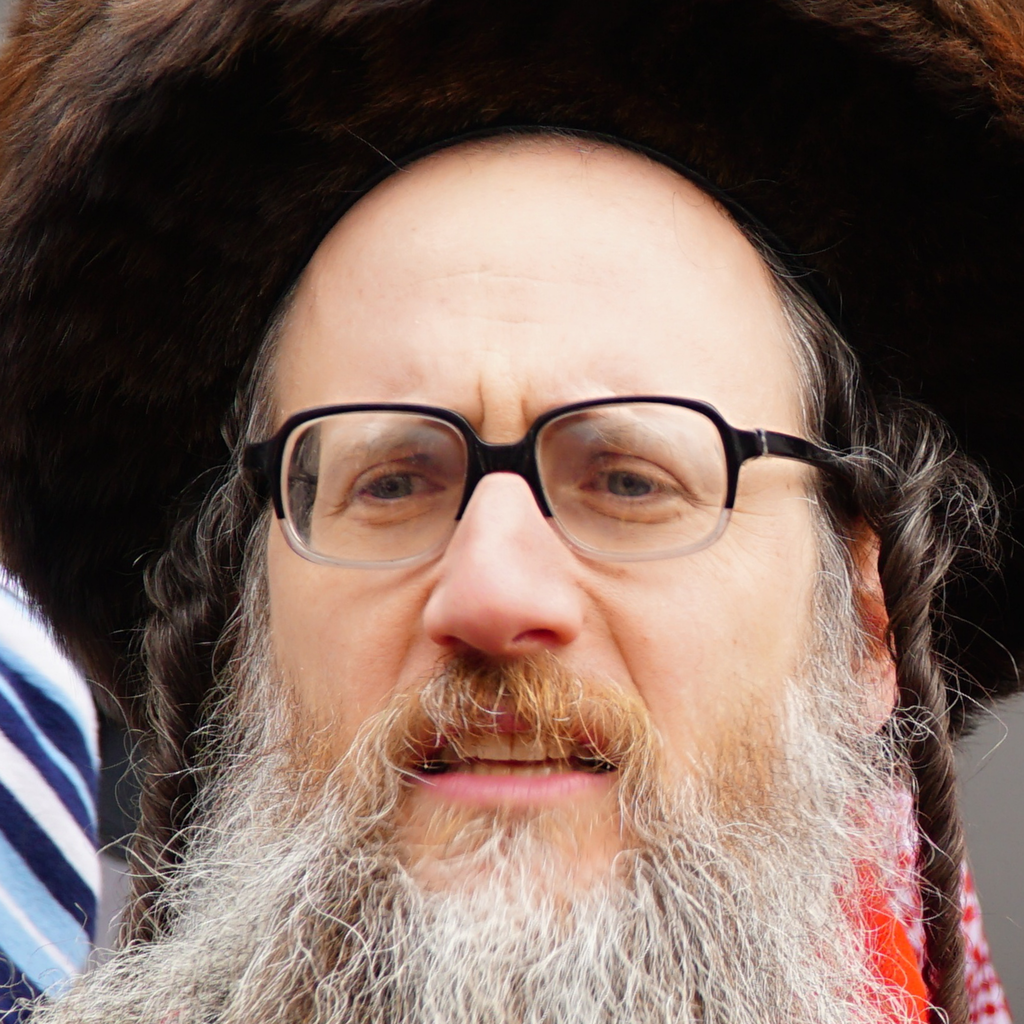
\includegraphics[width=.19\textwidth]{figures/66000.png}} \quad
    \subfloat[][\emph{Artline's output}]
    {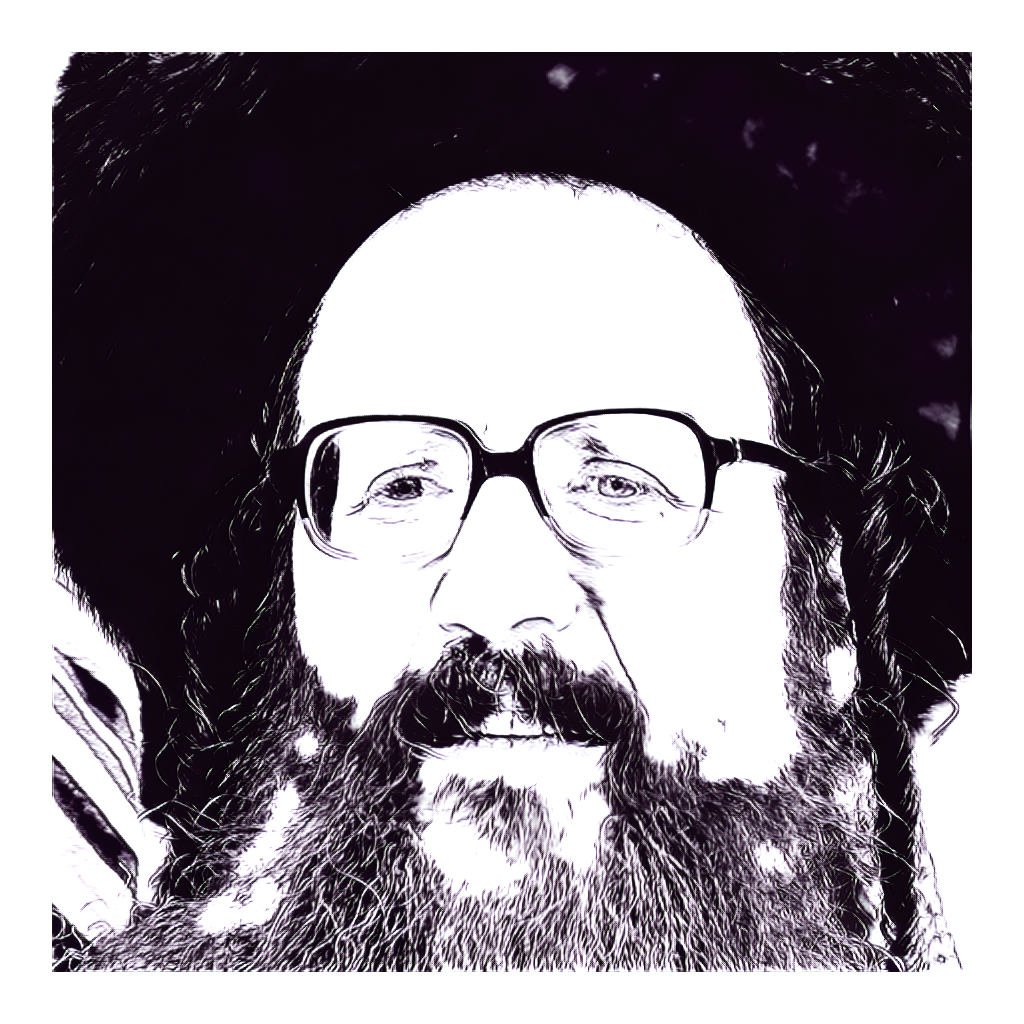
\includegraphics[width=.2\textwidth]{figures/66000Artile.png}} \\
    \subfloat[][\emph{Original image}]
    {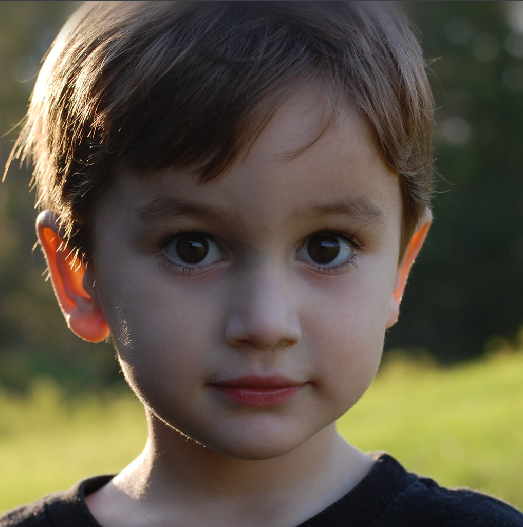
\includegraphics[width=.19\textwidth]{figures/66006.png}} \quad
    \subfloat[][\emph{Artline's output}]
    {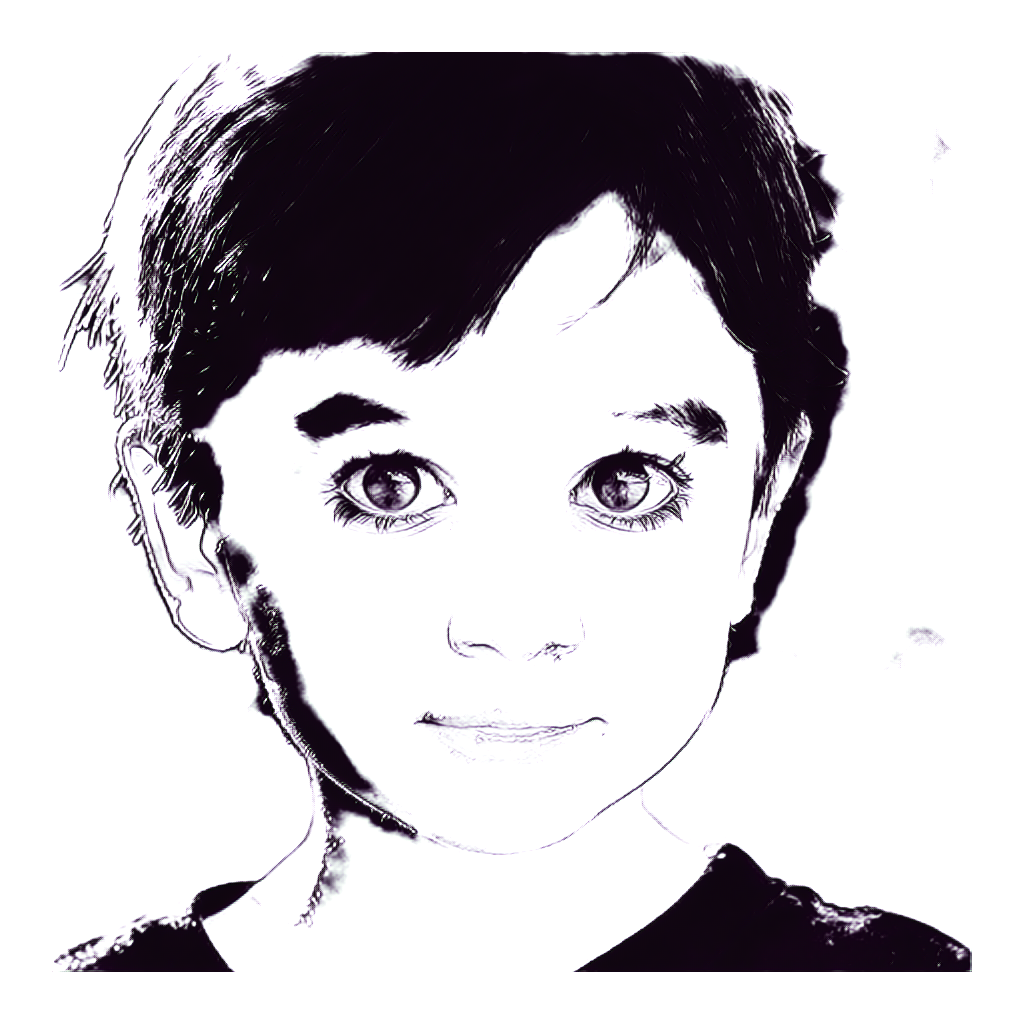
\includegraphics[width=.2\textwidth]{figures/66006-Artline.png}}
    \caption{Example of outputs obtained by using Artline}
    \label{fig:artlineRes}
\end{figure}
\noindent The performance of the four different models was evaluated and compared. The results of these models can be visualised in fig. \ref{fig:simplifyModelsRes}. The aim of this evaluation was to determine which model provided the best results for the desired application. After thorough testing, it was discovered that the MSE+GAN model and the model pencil1 both offered remarkable results, even if in different scenarios. The Artline network, as already specified, had the tendency to produce images with a high number of dark pixels, particularly in areas such as hair, facial hair and sometimes even in the background. To address this issue, the model to be used was selected based on the number of dark pixels present in the image. When the image had less than 800,000 dark pixels, the MSE+GAN model was utilised. On the other hand, for images with more dark pixels, the model pencil1 was applied.
\begin{figure}[htbp]
    \centering
    \subfloat[][\emph{MSE model}]
    {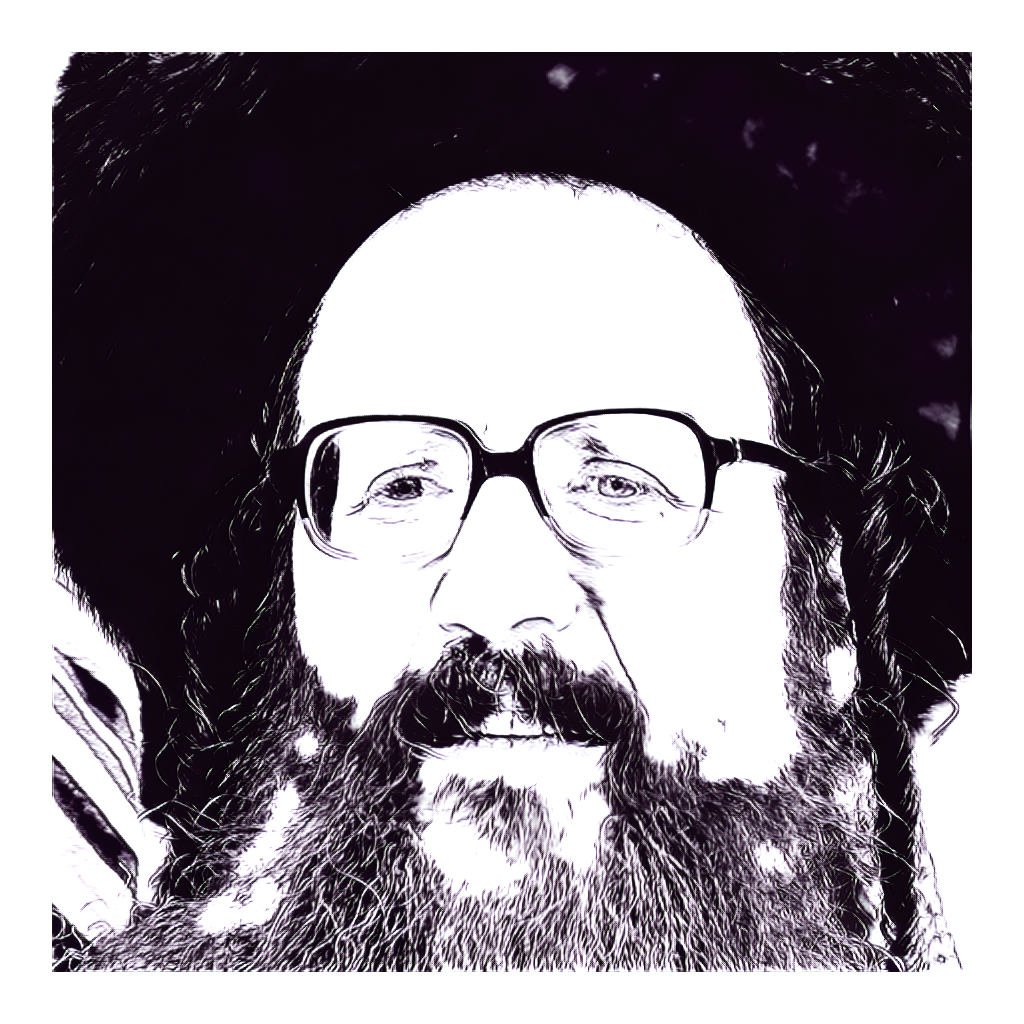
\includegraphics[width=.22\textwidth]{figures/66000Artile.png}} \quad
    \subfloat[][\emph{MSE + GAN model}]
    {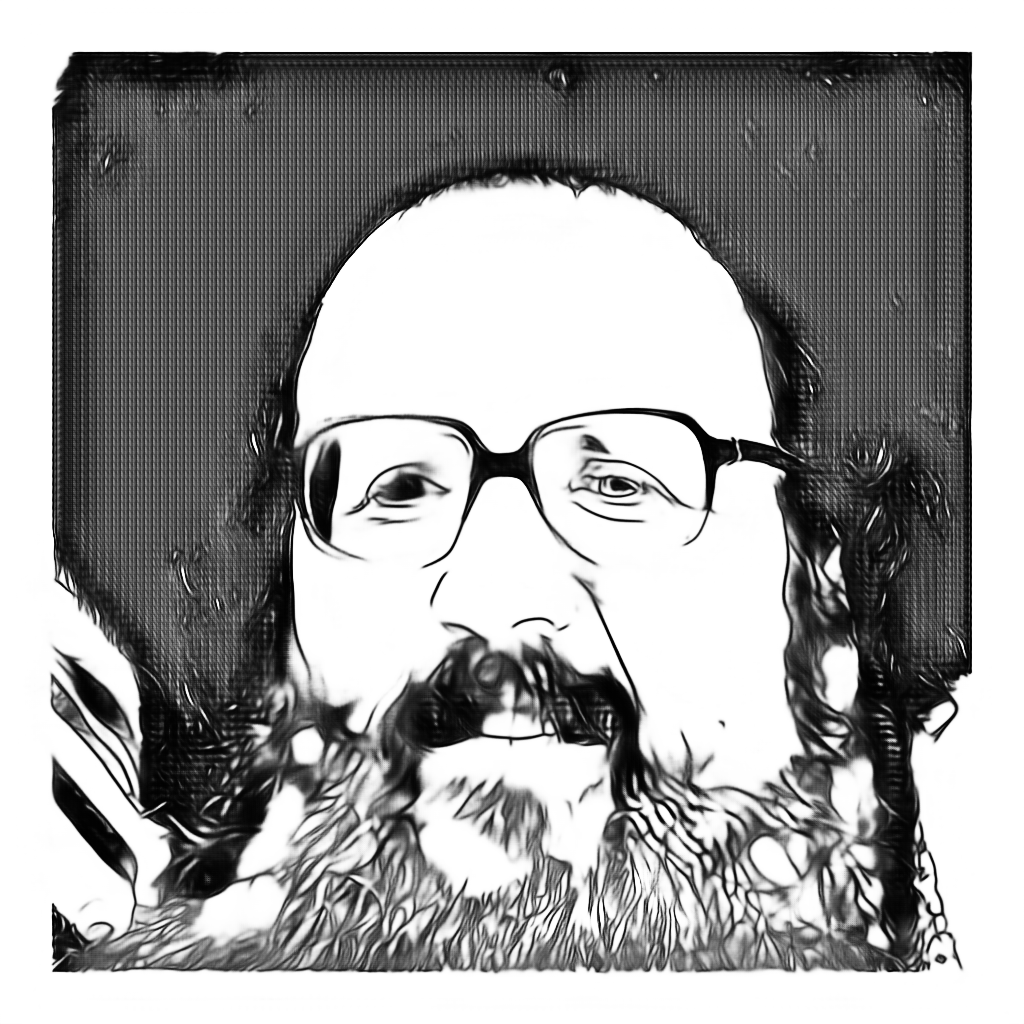
\includegraphics[width=.22\textwidth]{figures/66000mse.png}}
    \subfloat[][\emph{pencil1 model}]
    {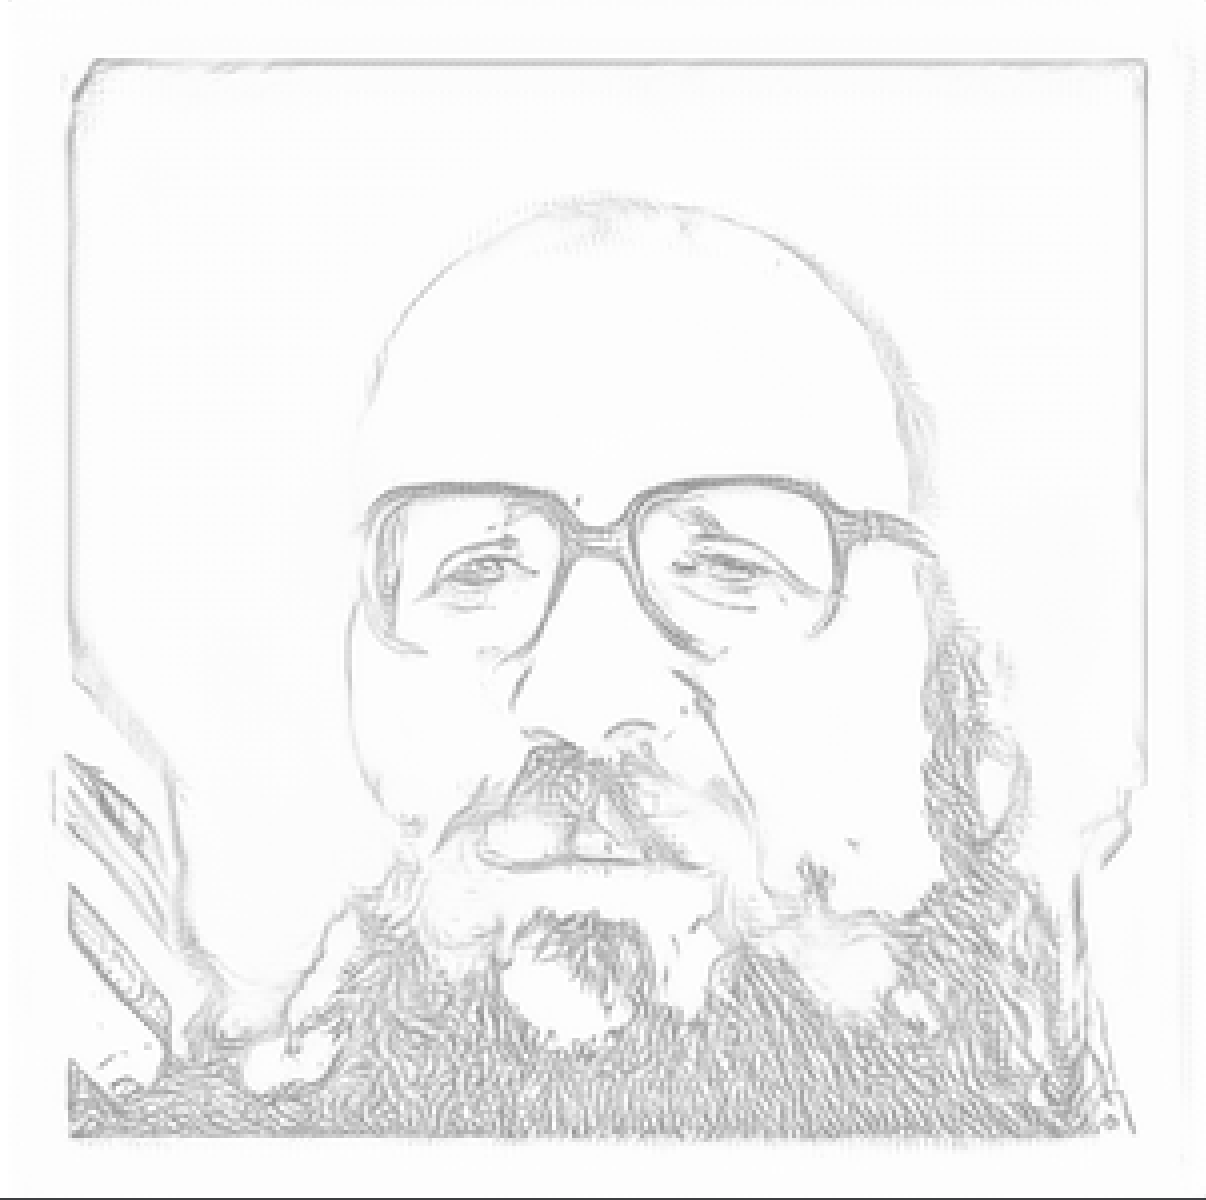
\includegraphics[width=.22\textwidth]{figures/66000-pencil1.png}}
    \subfloat[][\emph{pencil2 model}]
    {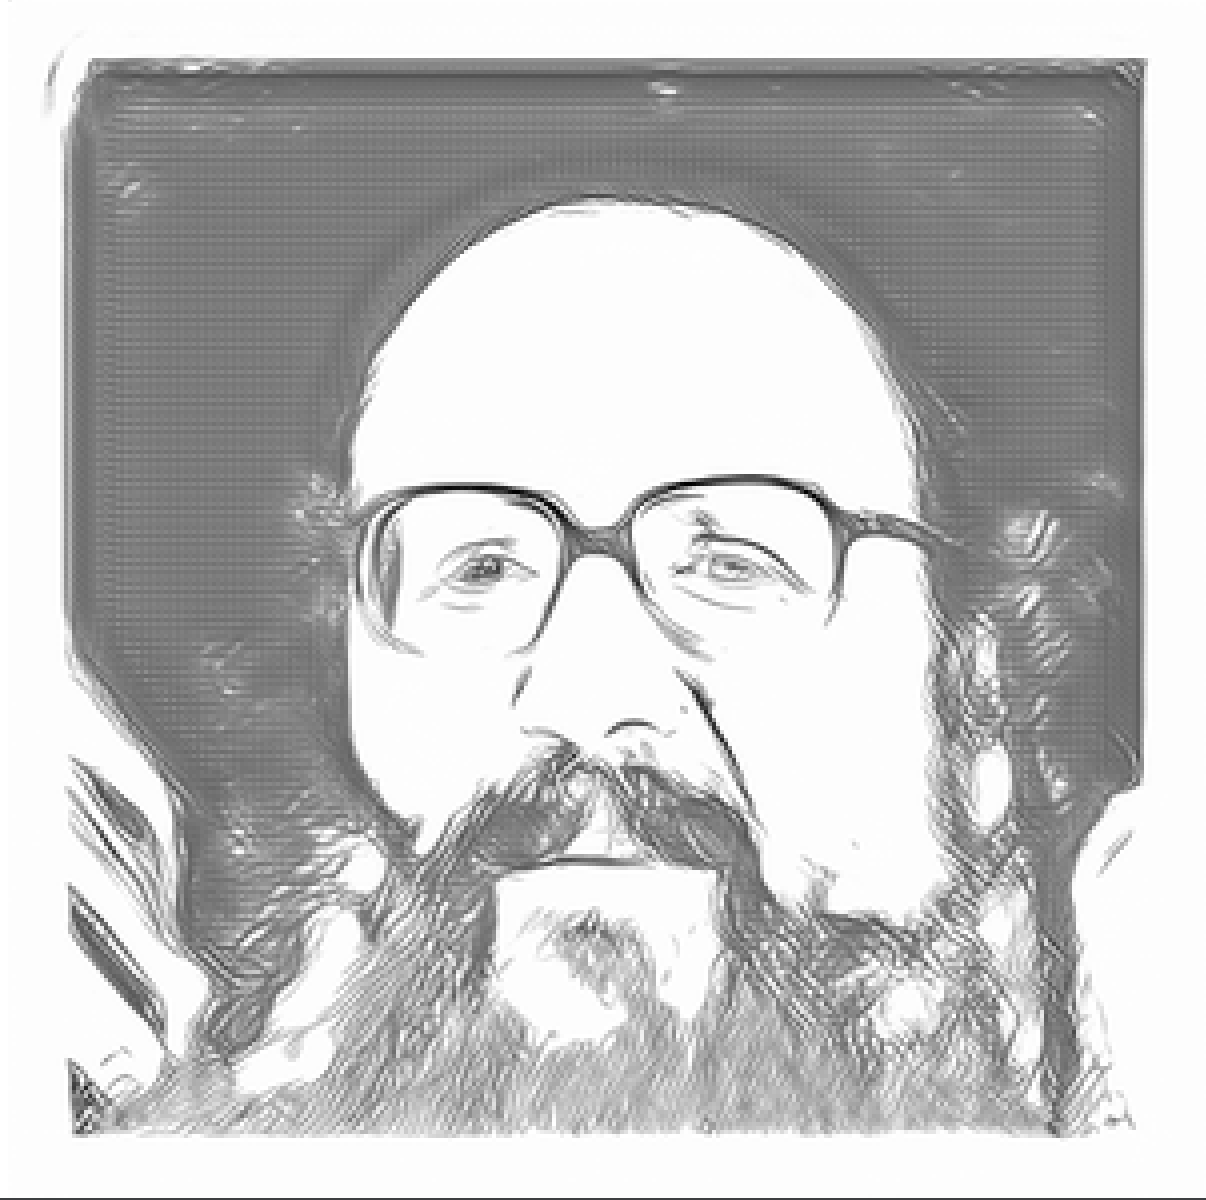
\includegraphics[width=.22\textwidth]{figures/66000-pencil2.png}}\\
    \subfloat[][\emph{MSE model}]
    {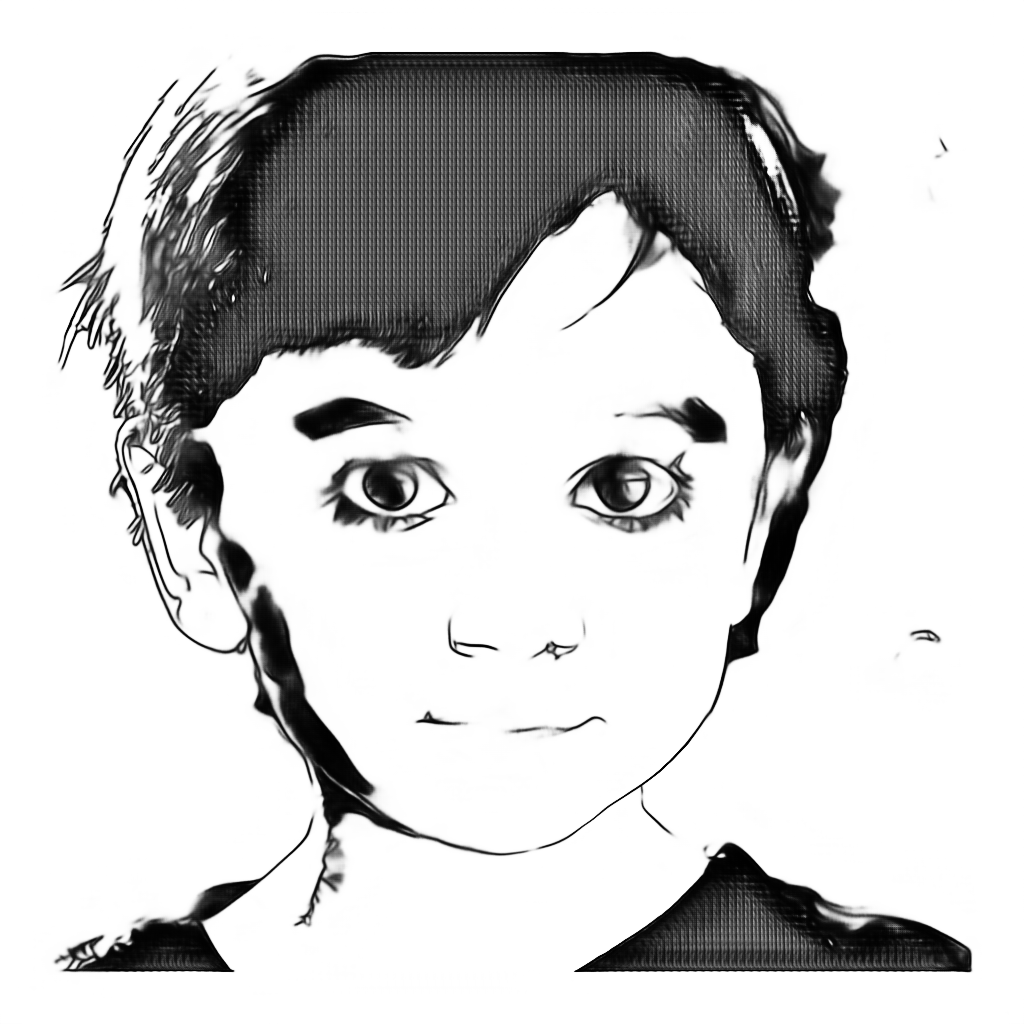
\includegraphics[width=.22\textwidth]{figures/66006-mse.png}} \quad
    \subfloat[][\emph{MSE + GAN model}]
    {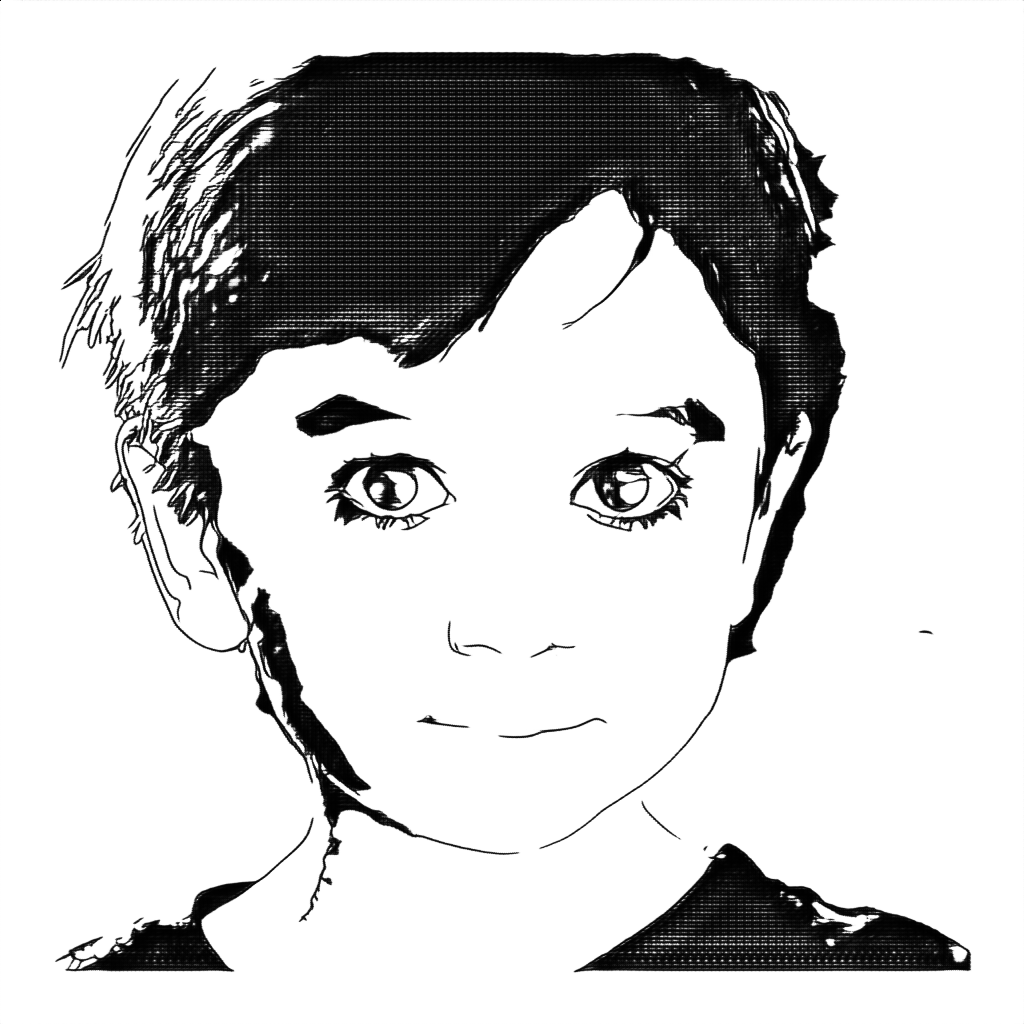
\includegraphics[width=.22\textwidth]{figures/66006-gan.png}}
    \subfloat[][\emph{pencil1 model}]
    {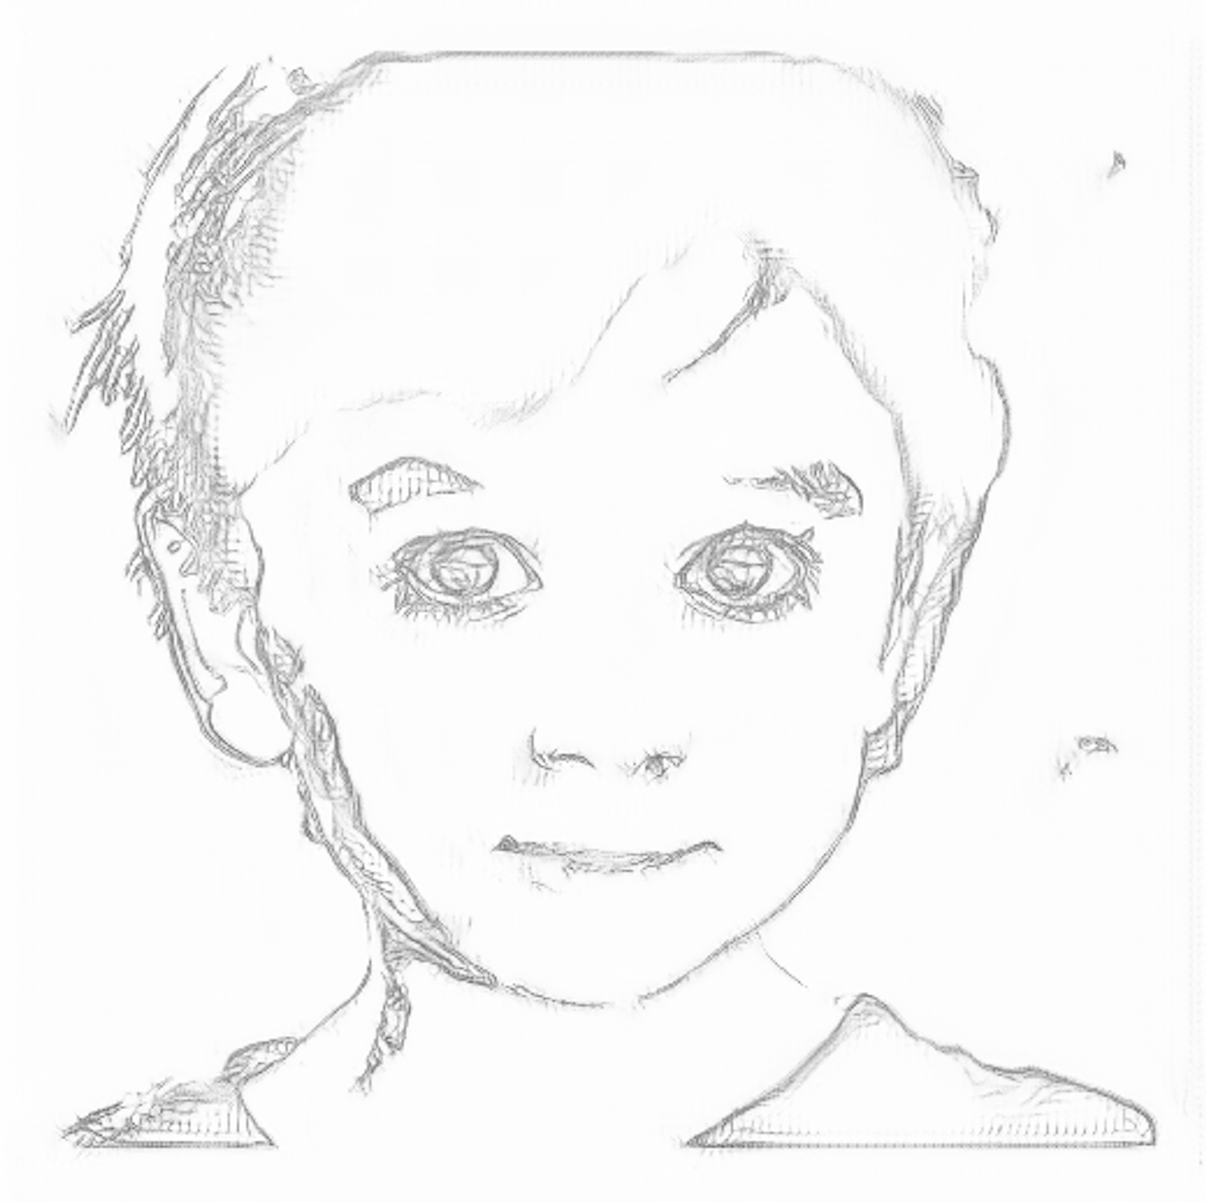
\includegraphics[width=.22\textwidth]{figures/66006-pencil1.png}}
    \subfloat[][\emph{pencil2 model}]
    {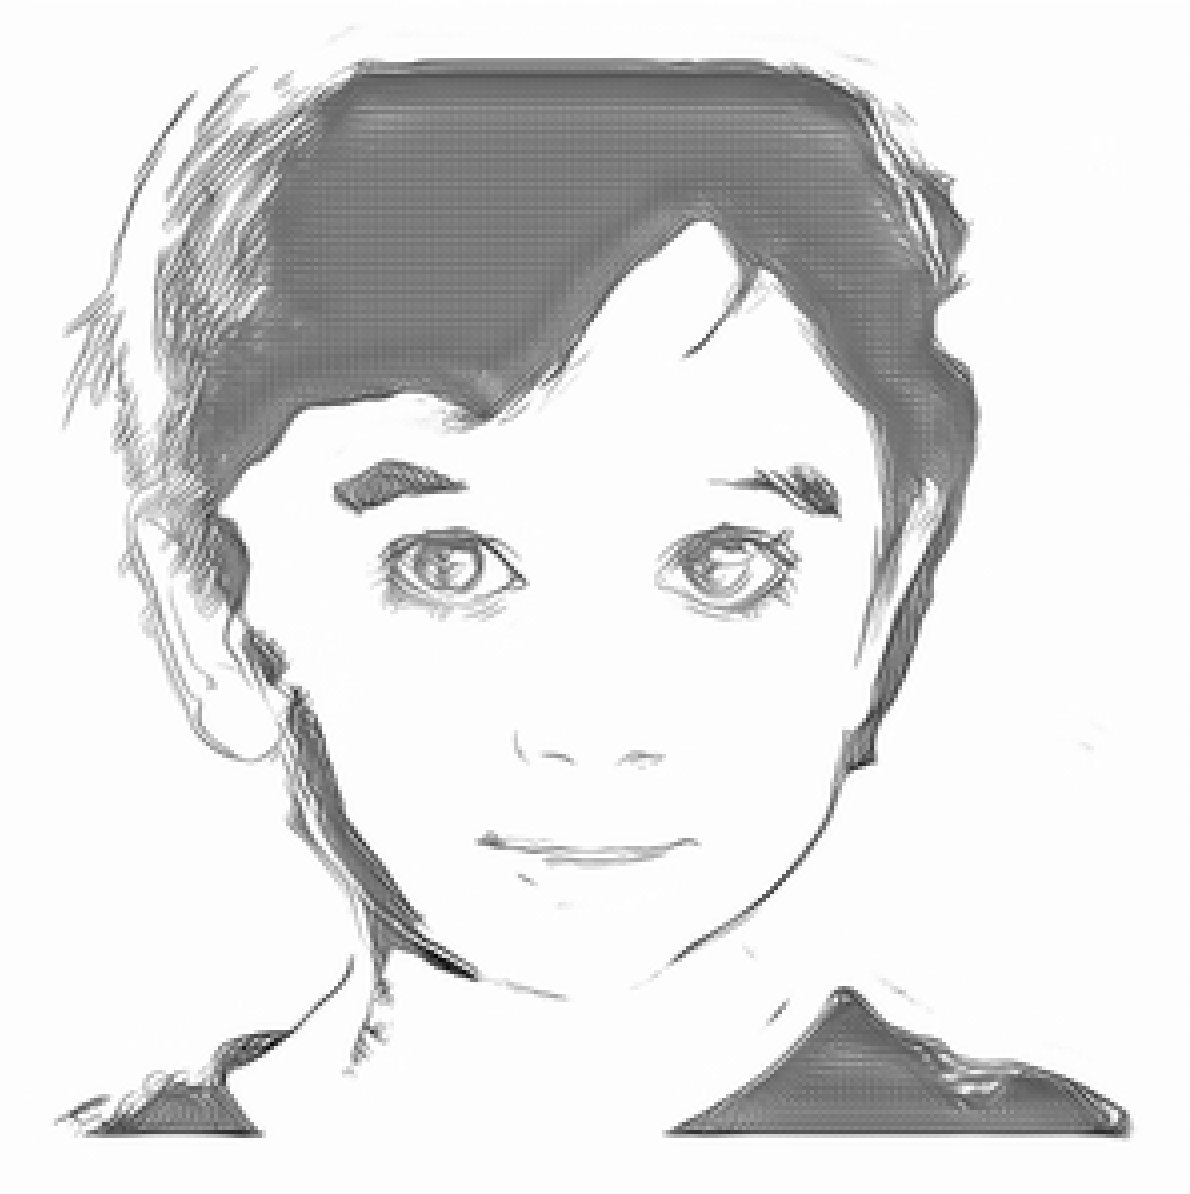
\includegraphics[width=.22\textwidth]{figures/66006-pencil2.png}}
    \caption{Output image obtained applying Artline and one of the four models of Learning to Simplify}
    \label{fig:simplifyModelsRes}
\end{figure}

\noindent After undergoing these two steps, the dataset obtained was lacking in quality as several sketches had lost some key facial features, such as lines of the lips or wrinkles. Applying the Learning to Simplify method to simplify the results from the Artline network was not the optimal solution, as Learning to Simplify is designed to convert rough sketches into clean, simplified drawings. The outcome of the network training phase responsible for generating a photo of a face from a sketch was disappointing, despite the network being trained for several days. This was due to the low quality of the dataset, which resulted in an insufficient number of high-quality sketches. To overcome this disappointment, further improvements to the dataset were required to ensure that it captured the necessary features for producing accurate facial sketches.

\noindent The new approach considered was a two-step procedure, starting with the application of an edge detection operator and then simplifying the results. While there are many available edge detection algorithms, they each have their own strengths and weaknesses. However, not all of them were suitable for this particular task, as the goal was not only to extract edges but also to produce results that resemble an artist’s sketch. Hence, the edge detector operator chosen is the XDoG operator. The results obtained with this operator are much more like drawings made by artists and are far better the one obtained using Artline. In fig. \ref{fig:xdogRes} can be seen the results of the operator used with these parameters:
\begin{itemize}
    \item $\epsilon = 0.01$
    \item $k = 200$
    \item $\sigma_1 = 0.05$,  $\sigma_2=k * \sigma_1 = 10$
    \item $\phi = 10$
\end{itemize}

\begin{figure}[htbp]
    \centering
    \subfloat[][\emph{}]
    {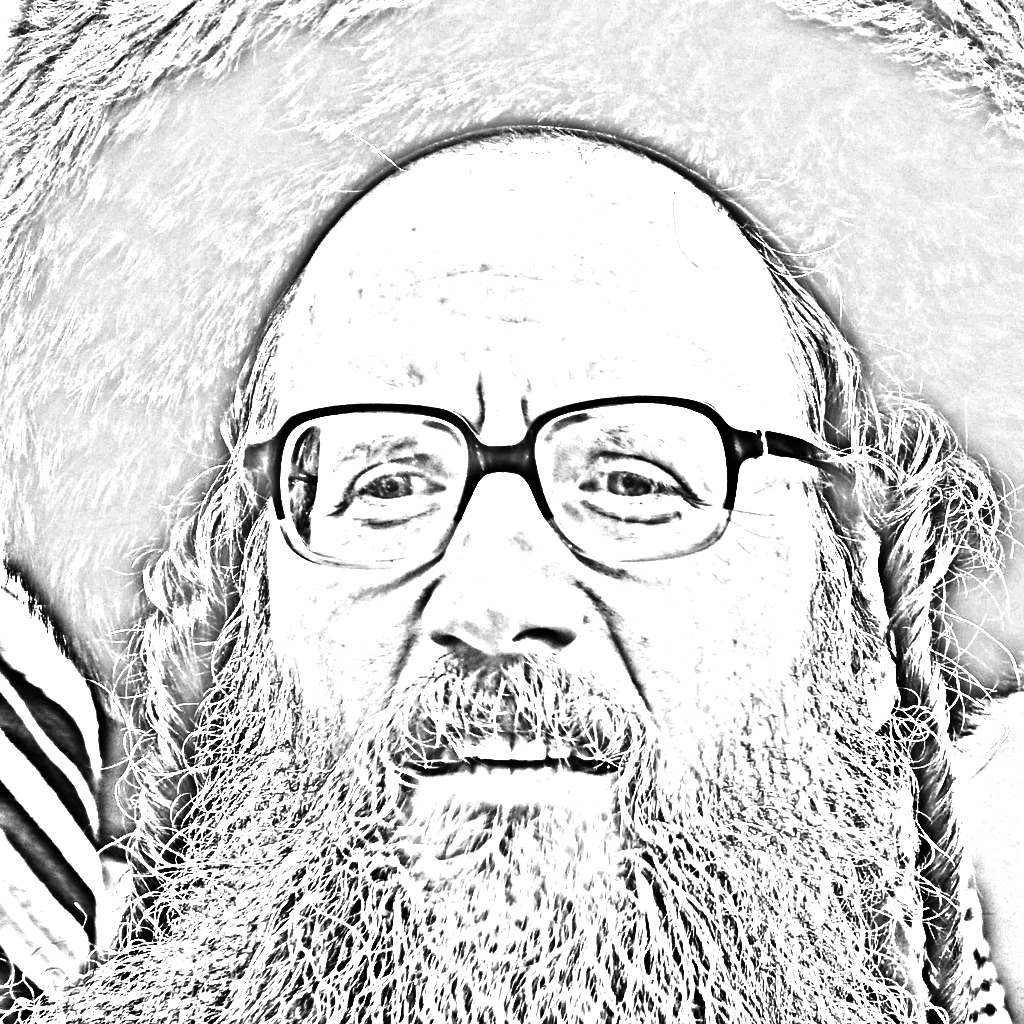
\includegraphics[width=.25\textwidth]{figures/66000-xdog.png}} \quad
    \subfloat[][\emph{}]
    {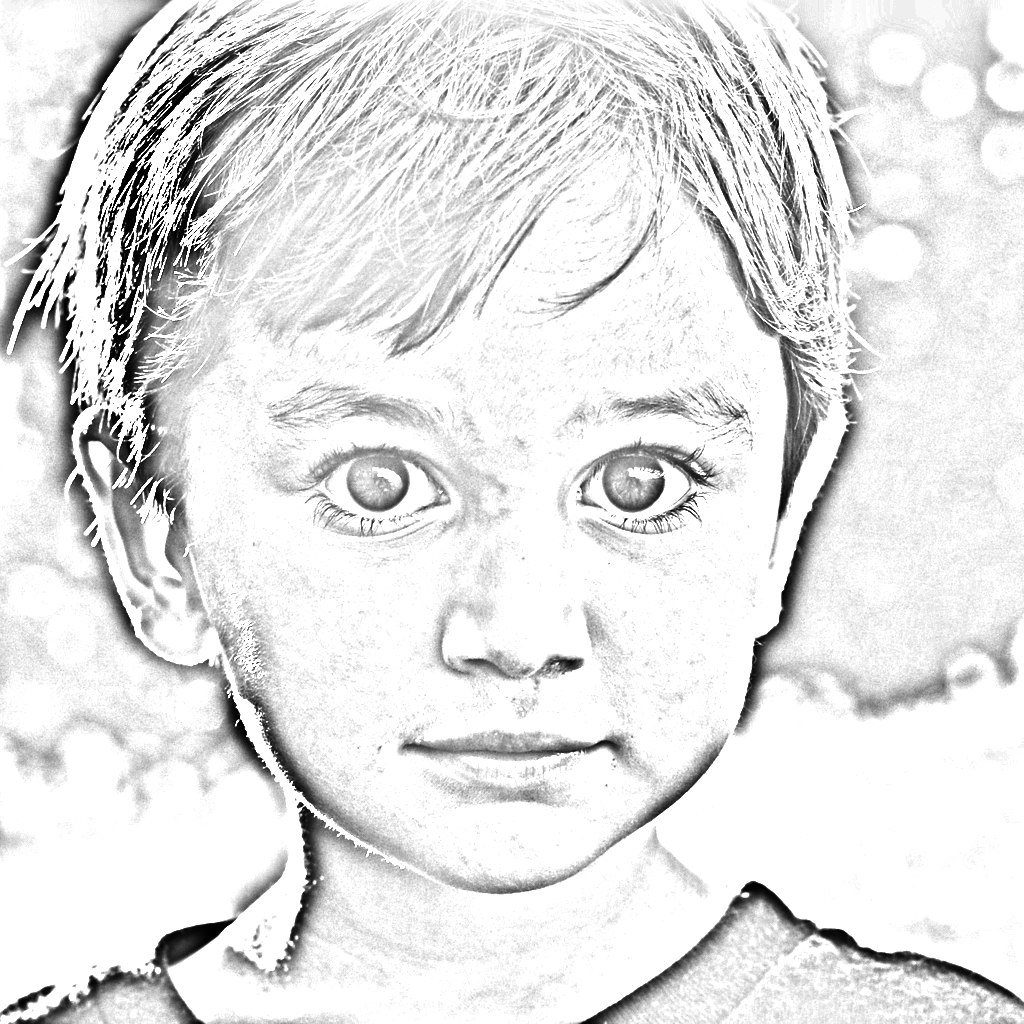
\includegraphics[width=.25\textwidth]{figures/66006-xdog.png}}
    \caption{Output image obtained applying the XDoG operator}
    \label{fig:xdogRes}
\end{figure}

\noindent Even if the results were very good, Learning to Simplify was applied in order to simplify the “sketches”. The results had to be simplified as well because the final goal is to obtain a photo of a face even if a person with no drawing ability does a sketch.
The result of this further step can be seen in fig. \ref{fig:xdogSimplifyRes}, they are significantly better compared to the ones obtained from the first approach, and it can be seen that there are preserved a lot of details that were lost in the first approach. 

\begin{figure}[htbp]
    \centering
    \subfloat[][\emph{}]
    {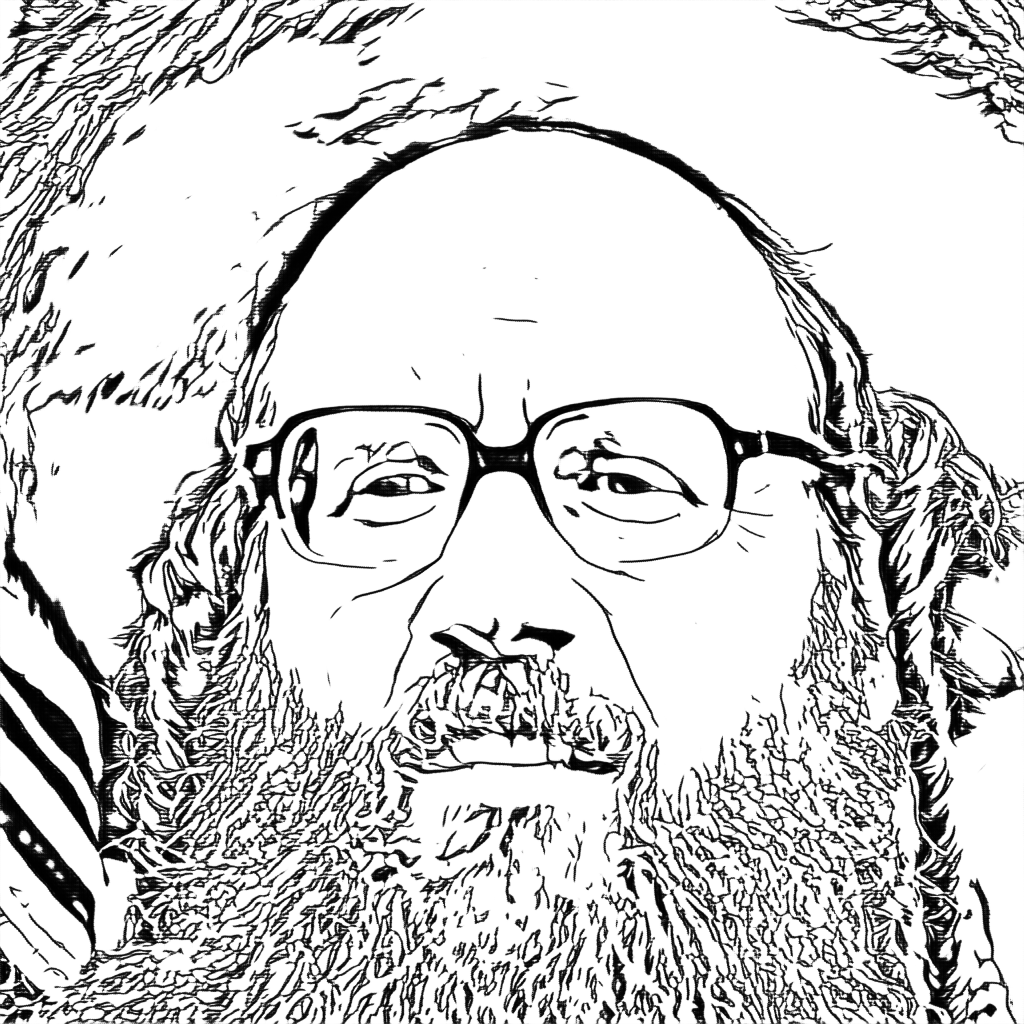
\includegraphics[width=.25\textwidth]{figures/66000-xdog-simplify.png}} \quad
    \subfloat[][\emph{}]
    {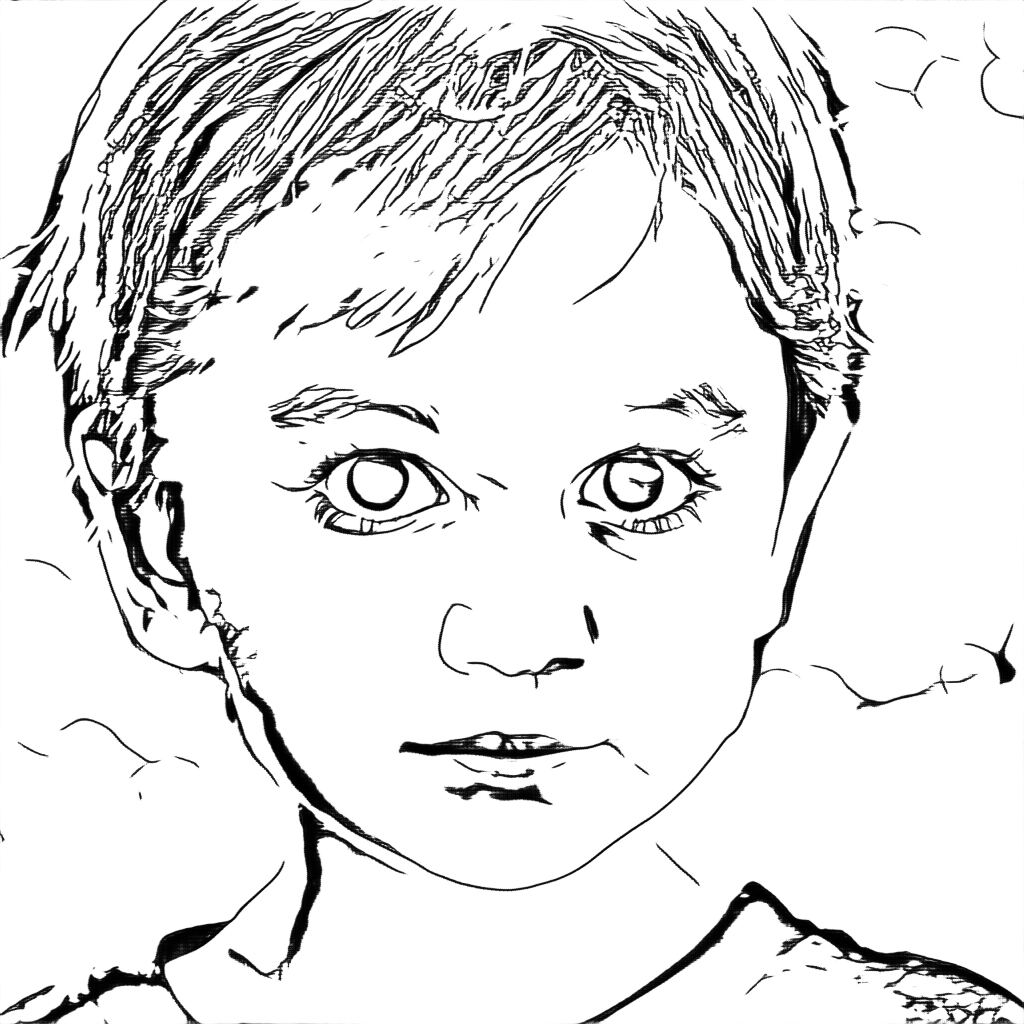
\includegraphics[width=.25\textwidth]{figures/66006-xdog-simplify.png}}
    \caption{Output image obtained applying Learning to Simplify to the output image of XDoG operator}
    \label{fig:xdogSimplifyRes}
\end{figure}